\begin{frame}[t]{Programa}
\vspace{-9mm}
\begin{block}{}
\begin{itemize}
\item Desenvolvimento todo em MATLAB.
\vspace{1mm}
\item Métodos de minímos feitos na forma de funções.
\vspace{1mm}
\item Interface gráfica feita com a ferramenta GUIDE.
\end{itemize}
\vspace{-3mm}
\begin{figure}[H]
	\begin{center}
		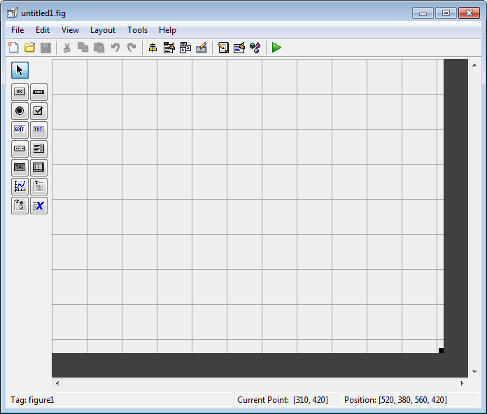
\includegraphics[width=5cm]{GUIDE}   
		\vspace{-0.15cm}
		\caption{Ambiente de desenvolvimento de interface gráfica}
		\label{fig:GUIDE}
	\end{center}
\end{figure}

\end{block}
\end{frame}
\begin{frame}{}
\vspace{0mm}
\hspace{4mm}
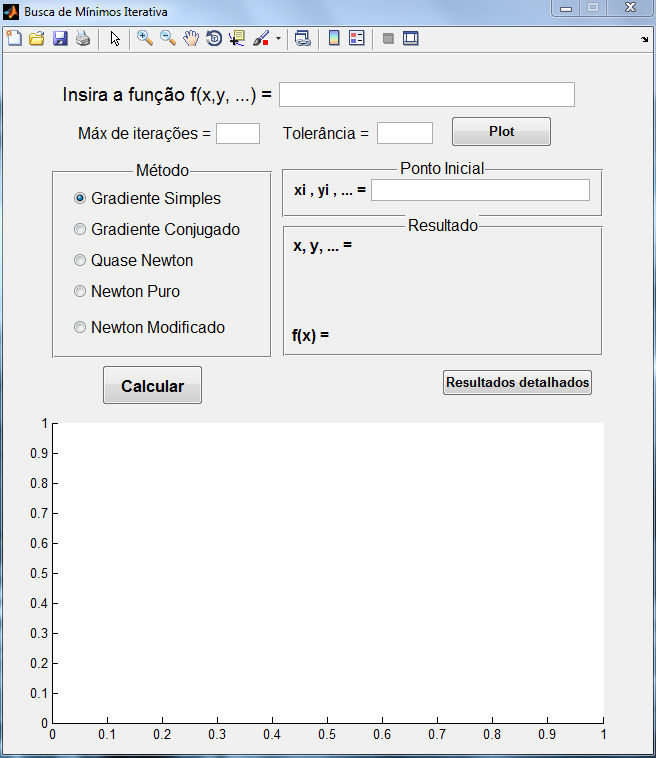
\includegraphics[scale=0.55]{GUI}
\end{frame}